\documentclass[11pt]{article}
\usepackage{graphicx, enumerate, amsmath}
\usepackage{tabularx}
\graphicspath{ {./img/} }
\parindent 0px
\date{February 16, 2024}
\title{CS 362 :\hspace{2px}: Homework 2}
\author{Ryan Magdaleno}

% Helpful ::
% \line(1,0){358px}

\begin{document}
\maketitle

%%%%%%%%%%%%%%%%%%%%%%%%%%%%%%%%%%%%%%%%%%%%%%%%%%%%%%%%%%%%%%%%%%%%%%%%%%%%%%%%%%%%%%%%%

\textbf{Problem 1.} Write the truth table for the CMOS Circuit given below and specify 
which logic gate it represents.

\vspace{5px}\textbf{Solution ::}
\begin{enumerate}[a)]
    \item ::
    \begin{center}
        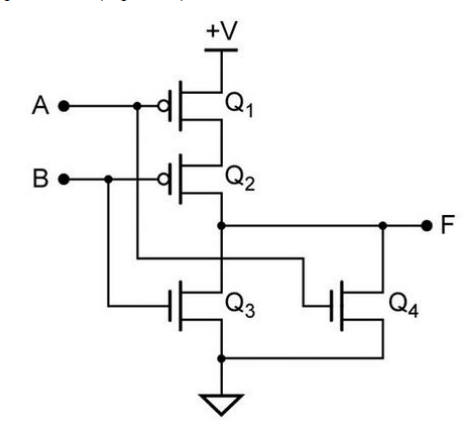
\includegraphics[scale=0.7]{1a.png}
    \end{center}
    \begin{center}
    \begin{tabularx}{0.7\textwidth} { 
        | >{\centering\arraybackslash}X 
        | >{\centering\arraybackslash}X 
        | >{\centering\arraybackslash}X 
        | >{\centering\arraybackslash}X 
        | >{\centering\arraybackslash}X 
        | >{\centering\arraybackslash}X 
        | >{\centering\arraybackslash}X | }
        \hline  $A$ & $B$ & $Q_1$ & $Q_2$ & $Q_3$ & $Q_4$ & $F$ \\
        \hline  0 & 0 & 1 & 1 & 0 & 0 & 1 \\
        \hline  0 & 1 & 1 & 0 & 1 & 0 & 0 \\
        \hline  1 & 0 & 0 & 1 & 0 & 1 & 0 \\
        \hline  1 & 1 & 0 & 0 & 1 & 1 & 0 \\
        \hline
    \end{tabularx}
    \end{center}
    This circuit represents a NOR gate.
    \pagebreak

    \item ::
    \begin{center}
        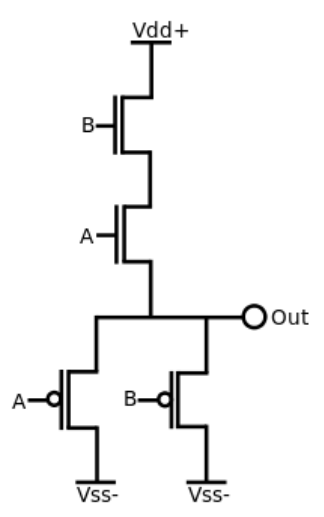
\includegraphics[scale=0.7]{1b.png}
    \end{center}
    \begin{center}
        \begin{tabularx}{0.35\textwidth} { 
            | >{\centering\arraybackslash}X 
            | >{\centering\arraybackslash}X 
            | >{\centering\arraybackslash}X | }
            \hline  $A$ & $B$ & Out \\
            \hline  0 & 0 & 0 \\
            \hline  0 & 1 & 0 \\
            \hline  1 & 0 & 0 \\
            \hline  1 & 1 & 1 \\
            \hline
        \end{tabularx}
    \end{center}
    This circuit represents an AND gate.
\end{enumerate}
\pagebreak
Write the truth table for the CMOS Circuit given below and specify 
the equation it represents.
\begin{enumerate}[a)]
    \item ::
    \begin{center}
        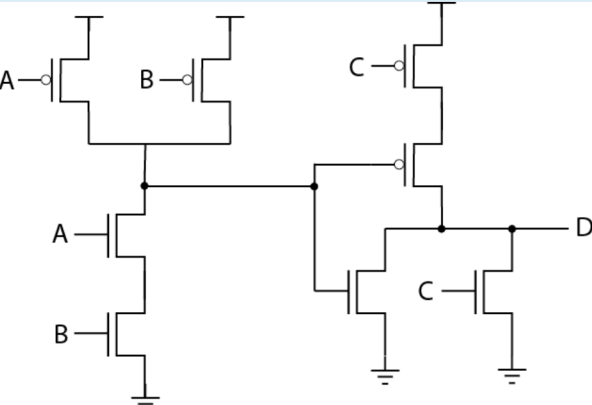
\includegraphics[scale=0.7]{1c.png}
    \end{center}
    \begin{center}
        \begin{tabularx}{0.35\textwidth} { 
            | >{\centering\arraybackslash}X 
            | >{\centering\arraybackslash}X 
            | >{\centering\arraybackslash}X 
            | >{\centering\arraybackslash}X | }
            \hline  $A$ & $B$ & $C$ & $D$ \\
            \hline  0 & 0 & 0 & 0 \\
            \hline  0 & 0 & 1 & 0 \\
            \hline  0 & 1 & 0 & 0 \\
            \hline  0 & 1 & 1 & 0 \\
            \hline  1 & 0 & 0 & 0 \\
            \hline  1 & 0 & 1 & 0 \\
            \hline  1 & 1 & 0 & 1 \\
            \hline  1 & 1 & 1 & 0 \\
            \hline
        \end{tabularx}
    \end{center}
    This circuit table can be represented like so:
    $$D = ABC'$$
    \pagebreak

    \item ::
    \begin{center}
        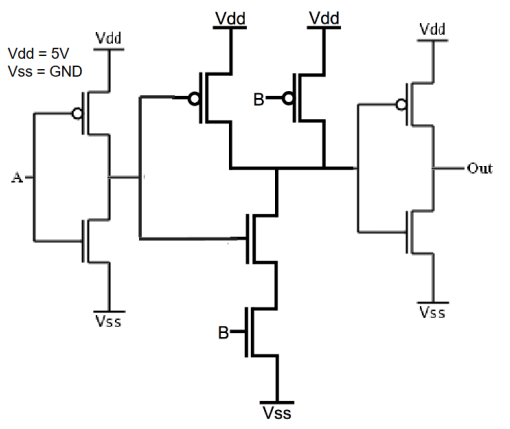
\includegraphics[scale=0.7]{1d.png}
    \end{center}
    \begin{center}
        \begin{tabularx}{0.35\textwidth} { 
            | >{\centering\arraybackslash}X 
            | >{\centering\arraybackslash}X 
            | >{\centering\arraybackslash}X | }
            \hline  $A$ & $B$ & Out \\
            \hline  0 & 0 & 0 \\
            \hline  0 & 1 & 1 \\
            \hline  1 & 0 & 0 \\
            \hline  1 & 1 & 0 \\
            \hline
        \end{tabularx}
    \end{center}
    This circuit table can be represented like so:
    $$Out = A'B$$
\end{enumerate}
\pagebreak

%%%%%%%%%%%%%%%%%%%%%%%%%%%%%%%%%%%%%%%%%%%%%%%%%%%%%%%%%%%%%%%%%%%%%%%%%%%%%%%%%%%%%%%%%

\textbf{Problem 2.} NAND gates and NOR gates are two types of Universal Gates.
Represent each equation as a circuit using only \textbf{a single type} of a
Universal Gate. I.E. Each answer must contain only NAND gates or must contain
only NOR gates. Assume literals are not available in complemented form.

\vspace{5px}\textbf{Solution ::}
\begin{enumerate}[a)]
    \item
    $F(x,y,z)=\overline{y}\,\overline{z} + \overline{y}z + \overline{x}y\overline{z}$
    \begin{center}
        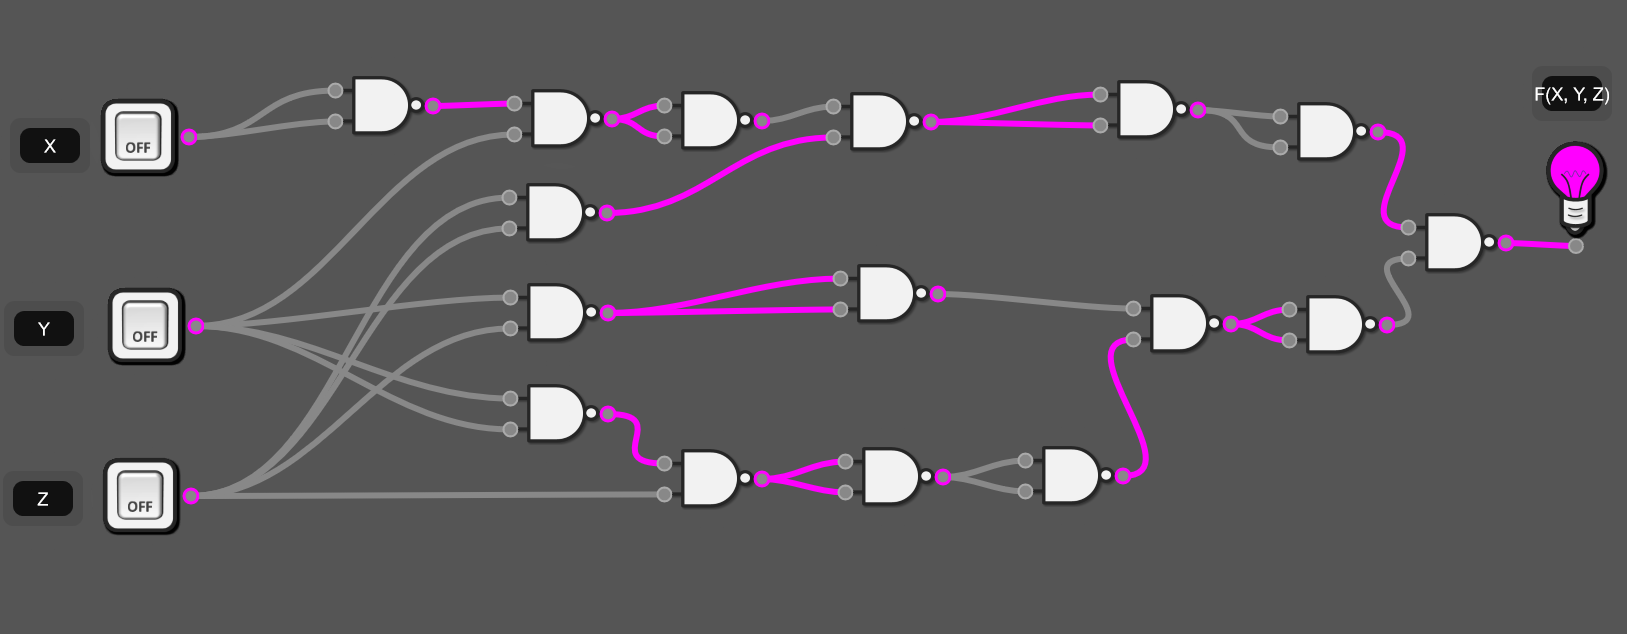
\includegraphics[scale=0.42]{2a.png}
    \end{center}
    \line(1,0){343px}

    \item
    $F(x,y,z) = (x' + y)\cdot(y+z)\cdot(x'+y'+z)$
    \begin{center}
        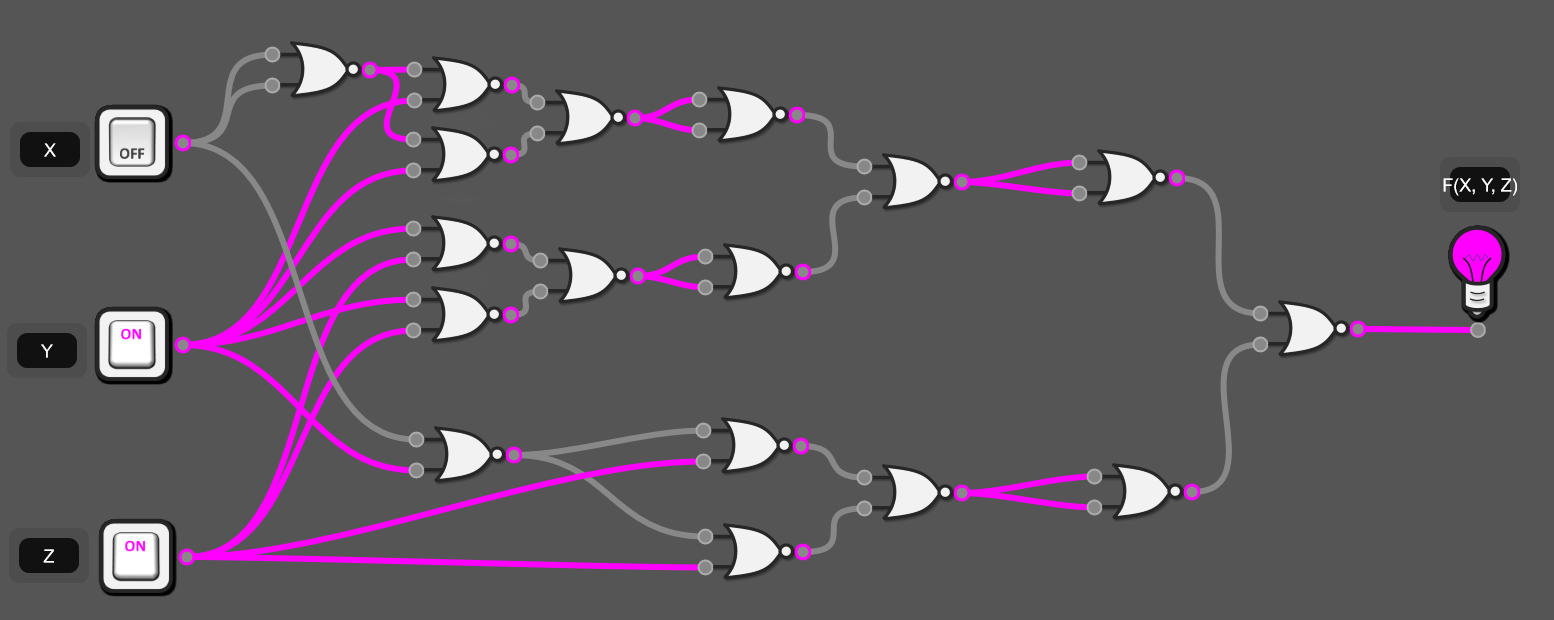
\includegraphics[scale=0.294]{2b.png}
    \end{center}
\end{enumerate}

\pagebreak

%%%%%%%%%%%%%%%%%%%%%%%%%%%%%%%%%%%%%%%%%%%%%%%%%%%%%%%%%%%%%%%%%%%%%%%%%%%%%%%%%%%%%%%%%

\textbf{Problem 3.} Write the truth table and equation for the following circuit
diagram. Do not do any simplification on the equation when written for your answer.
\begin{center}
    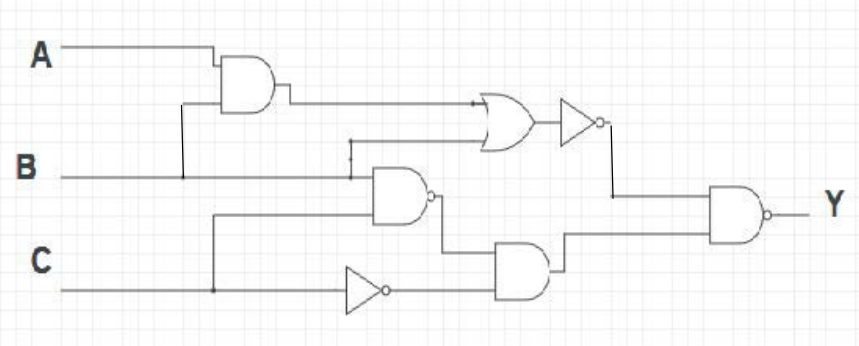
\includegraphics[scale=0.7]{3.png}
\end{center}

\vspace{5px}\textbf{Solution ::}
\begin{center}
    \begin{tabularx}{0.35\textwidth} { 
        | >{\centering\arraybackslash}X 
        | >{\centering\arraybackslash}X 
        | >{\centering\arraybackslash}X 
        | >{\centering\arraybackslash}X | }
        \hline  $A$ & $B$ & $C$ & $Y$ \\
        \hline  0 & 0 & 0 & 0 \\
        \hline  0 & 0 & 1 & 1 \\
        \hline  0 & 1 & 0 & 1 \\
        \hline  0 & 1 & 1 & 1 \\
        \hline  1 & 0 & 0 & 0 \\
        \hline  1 & 0 & 1 & 1 \\
        \hline  1 & 1 & 0 & 1 \\
        \hline  1 & 1 & 1 & 1 \\
        \hline
    \end{tabularx}
\end{center}
Equation:
$$Y = ABC + ABC' + AB'C + A'BC + A'BC' + A'B'C $$



\pagebreak

The following Boolean Properties are to be used and referenced by name for
each/every step to receive full credit when you “show your work” during the
remaining problems in this homework.
\begin{align*}
    a\cdot(b+c)=a\cdot+a\cdot c &= \text{Distributive (AND)} \\
    a+(b\cdot c)=(a+b)\cdot(a+c) &= \text{Distributive (OR)} \\
    a\cdot b = b\cdot a  &= \text{Commutative} \\
    a+b=b+a& \\
    (a\cdot b)\cdot c=a\cdot (b\cdot c)&= \text{Associative} \\
    (a+b)+c = a+(b+c)& \\
    a\cdot a' = 0 &= \text{Complement (AND)} \\
    a + a' = 1&= \text{Complement (OR)} \\
    a\cdot 1=a&= \text{Identity (AND)} \\
    a + 0 = a&= \text{Identity (OR)} \\
    a\cdot 0 = 0&= \text{Null elements} \\
    a + 1 = 1& \\
    a\cdot a=a&= \text{Idempotent} \\
    a + a = a& \\
    (a')' = a &= \text{Involution} \\
    (a\cdot b)' = (a'+b')&= \text{DeMorgan's (AND)} \\
    (a+b)' = (a'\cdot  b')&= \text{DeMorgan's (OR)}
\end{align*}
\pagebreak

%%%%%%%%%%%%%%%%%%%%%%%%%%%%%%%%%%%%%%%%%%%%%%%%%%%%%%%%%%%%%%%%%%%%%%%%%%%%%%%%%%%%%%%%%

\textbf{Problem 4.} Expand the following equations to sum--of--minterm equations

\vspace{5px}\textbf{Solution ::}
\begin{enumerate}[a)]
    \item
    $ab' + a'bc$ \hspace{20pt}(assume literals are $a,b,c$)
    \begin{align*}
        ab'(1) + a'bc &\text{\hspace{50pt}(Null elements)} \\
        ab'(c'+c) + a'bc &\text{\hspace{50pt}(Complement (OR))} \\
        ab'c + ab'c + a'bc &\text{\hspace{50pt}(Distributive (AND))}
    \end{align*}
    \line(1,0){343px}

    \item
    $ac + bc + a'b$ \hspace{5pt}(assume literals are $a,b,c$)
    \begin{align*}
        ac(1) + bc(1) + a'b(1)&\text{\hspace{30pt}(Null elements))} \\
        ac(b+b') + bc(a+a')+a'b(c'+c)&\text{\hspace{30pt}(Complement (OR))} \\
        ab'c + abc + abc + a'bc + a'bc' + a'bc &\text{\hspace{30pt}(Distributive (AND))}
    \end{align*}
    \line(1,0){343px}

    \item
    $ad'+b'c$ \hspace{25pt}(determine literals based on original equation)
    \begin{align*}
        ad'(1)(1)+b'c(1)(1) \\
        \text{\hspace{15pt}(Null elements)}& \\
        ad'(b+b')(c+c')+b'c(a+a')(d+d') & \\
        \text{\hspace{15pt}(Complement (OR))}& \\
        ad'(bc+bc'+b'c'+b'c)+b'c(a'd'+a'd+ad'+ad) \\
        \text{\hspace{15pt}(Distributive (AND))}& \\
        abcd'+abc'd'+abc'd'+ab'c'd'+ab'cd+ab'cd'+a'b'cd+a'b'cd' \\
        \text{\hspace{15pt}(Distributive (AND))}
    \end{align*}
\end{enumerate}
\pagebreak

%%%%%%%%%%%%%%%%%%%%%%%%%%%%%%%%%%%%%%%%%%%%%%%%%%%%%%%%%%%%%%%%%%%%%%%%%%%%%%%%%%%%%%%%%

\textbf{Problem 5.} Determine if the two equations ($y$ \& $z$) are equivalent by 
expanding each to a sum-of-minterm equation. Show your work. 

\vspace{5px}\textbf{Solution ::}
\begin{enumerate}[a)]
    \item 
    $y = ab'+a'b+c$ \\
    $z = ab'c'+ac+a'bc+a'c$
    \begin{align*}
        y &= ab'c+ab'c'+a'bc+a'bc'+a'b'c+a'bc'+ab'c+abc \\
        z &= a'b'c+a'bc+abc+ab'c+a'bc'+ab'c' \\
        &\text{$y$ and $z$ are equivalent equations.}
    \end{align*}
    \\\line(1,0){343px}

    \item 
    $y = a'b'+bc'$ \\
    $z = a'c'+b'c$
    \begin{align*}
        y &= a'bc'd' + a'bc'd + abc'd' + abc'd + a'b'c'd' + a'b'c'd + a'b'cd'
        + a'b'cd \\
        z &= a'b'cd' + a'b'cd + ab'cd' + ab'cd + a'b'c'd' + a'b'c'd + a'bc'd' + a'bc'd
        & \\
        y &= abc'd + abc'd' \\
        z &= ab'cd + ab'cd' \\
        &\text{$y$ and $z$ are not equivalent equations.}
    \end{align*}
\end{enumerate}
\pagebreak

%%%%%%%%%%%%%%%%%%%%%%%%%%%%%%%%%%%%%%%%%%%%%%%%%%%%%%%%%%%%%%%%%%%%%%%%%%%%%%%%%%%%%%%%%

\textbf{Problem 6a.} Convert the truth table to sum-of-minterms expression.\\
Show your work.
\begin{center}
    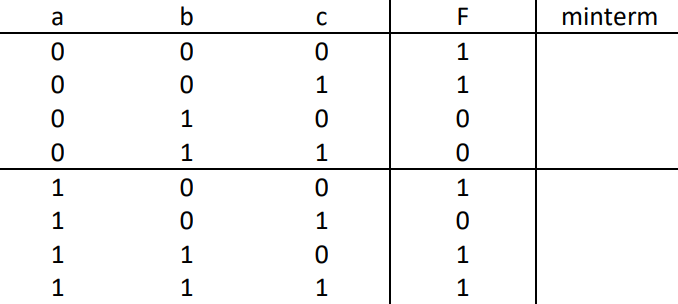
\includegraphics[scale=0.7]{6a.png}
\end{center}
\textbf{Solution ::}
\begin{align*}
    &= a'b'c' + a'b'c + ab'c' + abc' + abc\\
    &=(m_0 + m_1 + m_4 + m_6 + m_7) \\
    F(a,b,c) &= \sum \left(0, 1, 4, 6, 7\right)
\end{align*}
\pagebreak

\textbf{Problem 6b.} Convert the truth table to product-of-maxterms expression.\\
Show your work.
\begin{center}
    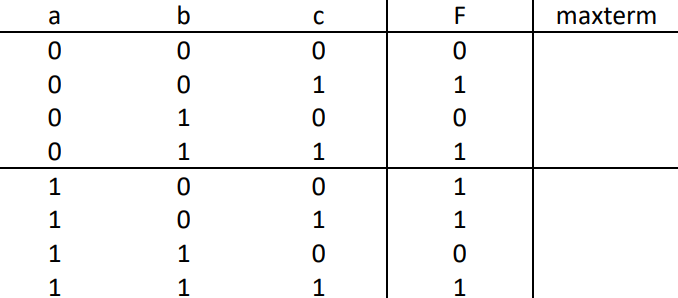
\includegraphics[scale=0.7]{6b.png}
\end{center}
\textbf{Solution ::}
\begin{align*}
    &= (a'+b'+c)\cdot(a+b'+c)\cdot(a+b+c) \\
    &= (M_0 \cdot M_2 \cdot M_6) \\
    F(a, b, c) &= \Pi M(0, 2, 6)
\end{align*}
\pagebreak

\textbf{Problem 6c.} Express the truth table to 
\textbf{either a sum-of-minterms expression or a product-of-maxterms expression.}
\\Choose the one with the simplest expression (i.e. fewest number of total literals). 
Show your work
\begin{center}
    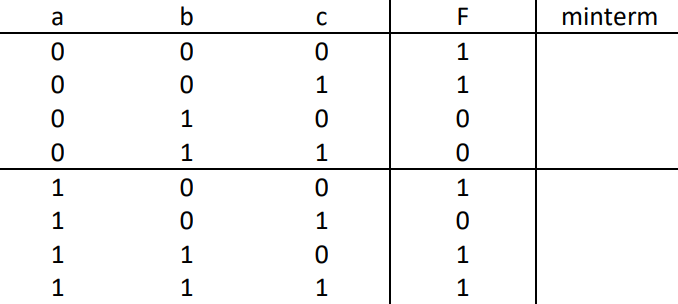
\includegraphics[scale=0.7]{6a.png}
\end{center}
\textbf{Solution ::}
\begin{align*}
    &= (a'+b+c' + (a+b+c)) \\
    &= (M_0\cdot M_5), \\
    F(a, b, c) &= \Pi M(0, 5)
\end{align*}
\pagebreak

\textbf{Problem 6d.} Express the truth table to either a sum-of-minterms expression
or a product-of-maxterms expression. Choose the one with the simplest expression
(i.e. fewest number of total literals). Show your work.
\begin{center}
    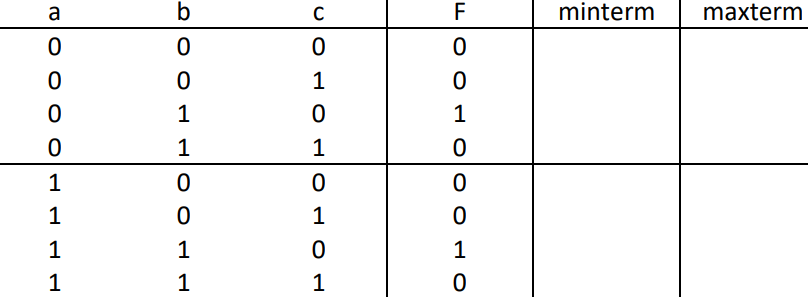
\includegraphics[scale=0.7]{6d.png}
\end{center}
\textbf{Solution ::}
\begin{align*}
    &= abc' + ab'c \\
    &= (m_2, m_6) \\
    F(a, b, c) &= \sum m(2, 6)
\end{align*}

\pagebreak

%%%%%%%%%%%%%%%%%%%%%%%%%%%%%%%%%%%%%%%%%%%%%%%%%%%%%%%%%%%%%%%%%%%%%%%%%%%%%%%%%%%%%%%%%

\textbf{Problem 7.} Simplify the sum-of-minterms expression below to sum-of-products
form using Boolean Algebra properties. The “simplest” expression has the fewest
literals. Show your work. (I'm super lost on this one)

\vspace{5px}\textbf{Solution ::}
\begin{enumerate}[a)]
    \item 
    $F(x,y,z) = x'y'z' + x'yz + xy'z' + xyz' + xyz$
    \begin{align*}
        &= x'yz + y'z'(x'+x)+xy(x'+z) \text{\hspace{15pt}Null elements and comp.
        (OR)}\\
        &= xy + y'z' + x'yz \\
        &= y(x'y + x) + y'z' \text{\hspace{15pt}Dist. (AND)}
    \end{align*}

    \line(1,0){343px}
    \item 
    $F(x,y,z)=  xyz' + x'y'z + x'y'z' + x'yz + x'yz'$
    \begin{align*}
        & xyz' + x'y'(x+z')+z'y(x+x') \\
        & xyz' + x'y'(1) + x'y(1) \text{\hspace{15pt}Null elements} \\
        & xyz' + x'y' + x'y \text{\hspace{15pt}complement (OR)}\\
        &x'y' + y(x' + z'x) \text{\hspace{15pt}Distributive (AND)}\\
        & x'y' + y((x+1)\cdot z') \text{\hspace{15pt}Null elements}\\
        & y'x  + z'y
    \end{align*}
\end{enumerate}
\vspace{200pt}: ( Ran out of time, 
\end{document}